\documentclass[12pt]{article}

\usepackage{color}
\usepackage[utf8]{inputenc}
\usepackage{indentfirst}
\usepackage{graphicx}
\usepackage{verbatim}
\usepackage{listings}
\usepackage{url}
\usepackage{stringenc}
\usepackage{pdfescape}
\usepackage{subfig}
\usepackage{float}
\begin{document}

\setlength{\textwidth}{16cm}
\setlength{\textheight}{22cm}
\title{\Huge\textbf{\textit{Scripting Languages}}\linebreak
\linebreak\linebreak\linebreak

\includegraphics[width=8cm]{feup.pdf}\linebreak \linebreak
\large{Mestrado Integrado em Engenharia Informática e Computação} \linebreak
\large{Desenvolvimento de Jogos de Computador \\ EIC0090-2S}\linebreak
}




\author{Daniel Borges Pereira - 201109110 (ei11132@fe.up.pt)\\
João Pedro Matos Teixeira Dias - 201106781 (ei11137@fe.up.pt)\\
José Pedro Vieira de Carvalho Pinto - 201203811 (ei12164@fe.up.pt)\\
\\\\\\\\\\ Faculdade de Engenharia da Universidade do Porto \\ Rua Roberto Frias, s\/n, 4200-465 Porto, Portugal
 \vspace{1cm}}
%\date{Junho de 2007}
\maketitle
\thispagestyle{empty}

%************************************************************************************************
%************************************************************************************************

\newpage

\tableofcontents

%************************************************************************************************
%************************************************************************************************

%*************************************************************************************************
%************************************************************************************************

\newpage

\newpage
\section{Introduction}

Given the choice made in the practical classes of DJCO (\textit{Desenvolvimento de Jogos de Computador}) of the theme for the game development assignment, scripting languages will be the major subject written on this report.

Scripting languages have been around for a few years and have now been gaining a bit more popularity amongst the more casual programmers but in games they have, for a while now, been there above the core games functions.

This report will cover the basics of scripting languages and their context in game development issuing some relevance to their advantages and disadvantages facing other types programming languages, mainly compiled languages. Topics such as its integration with other languages and platforms will also be covered as well as its access to more low level functions (e.g. in the case of game development).\newpage


\section{Scripting Languages - A Starting Point}
In terms of defining scripting languages there seems to be no precise conclusion but as a generalization we can say that they are high-level programming languages, less efficient but more flexible than compiled languages.

\begin{figure}[h!]
    \centering
    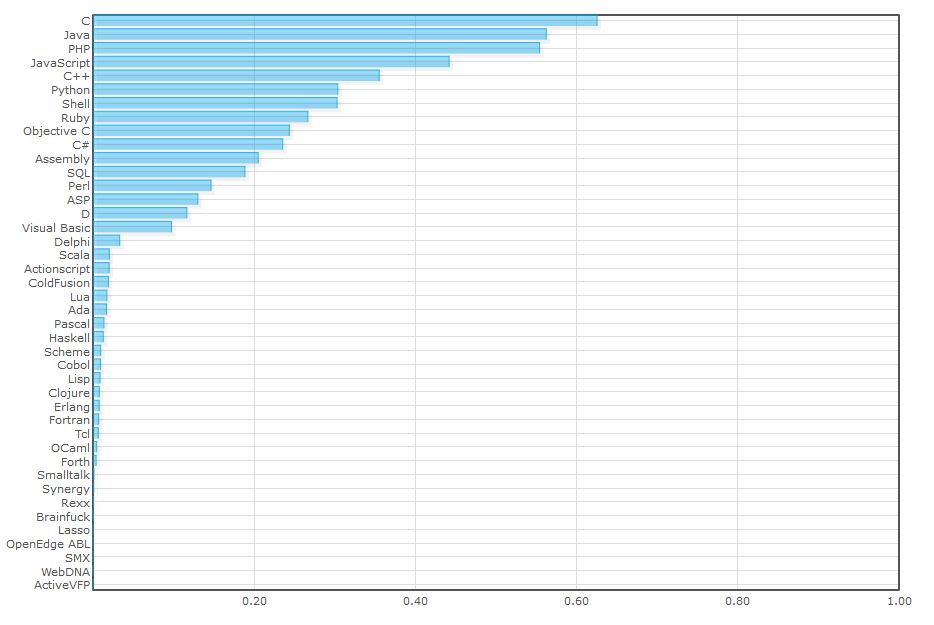
\includegraphics[width=0.8\textwidth]{pop.PNG}
    \caption{Some scripting languages appear as the most used programming languages in the rankings. Some examples are Python, Shell and Lua.}
    \label{fig:awesome_image}
\end{figure}

To be a bit more specific, there are a few characteristics that define or at least are true to most scripting languages, such as being Interpreted which as opposed to the compiled ones, allows for a quick turnaround during runtime and thus making applications more flexible.

They are Dynamically typed which makes them usually weakly typed, without prior restrictions on how a piece of data can be used, as well as encouraging reuse. Ruby for example has the “duck-typing” mechanism in which object types are determined by their runtime capabilities instead of by their class definition.

Scripting languages usually do not strongly separate data and code, and allow code to be created, changed, and added during runtime also, they are usually suited for flexible integration tasks and are supposed to be used in dynamic environments. Scripting languages usually allow strong reflection (the possibility to easily investigate data and code during runtime) and runtime interrogation of objects instead of relying on their class definitions.

\subsection{Proprieties of Scripting Languages}

Almost all scripting languages are cross-platform except for the ones that are specific to the operative system (Bash, PowerShell, AppleScript).

\begin{figure}[h!]
    \centering
    
\includegraphics[width=0.8\textwidth]{lol.jpg}
    \caption{\textit{League of Legends} screenshot. The minions and turrets behaviour in the game are known for being coded in Lua scripts.}
    \label{fig:awesome_image}
\end{figure}

The level of access of a scripting language to game engine can vary:
\begin{itemize}
\item When it's used to create a game the scripting language can interact directly with the game engine (when the game engine supports it).
\item When it's used  by the players the access is high-level, and may depend on the game and the implementation of it.
\end{itemize}

Scripting languages integrate very well into many languages, particularly with C/C++.

Today one of most used combinations are Lua scripting language and an engine written in C/C++. Examples of this are well-known games like \textit{League of Legends} and \textit{Sid Meier's Civilization V}.


\section{Between Scripting and Compiled languages}
At some point, with so many readily available, easy to use (and inexpensive or free) high-level scripting languages to choose from, why would anyone still resort to C, C++, or Java? We can think of several reasons, but execution speed and the desire to keep algorithms private are probably the dominant ones. Both of these reasons are going away, however, with increases in processor speed and the advent of compilers for traditionally interpreted scripting languages. \\

\emph{"It might seem that the typeless nature of scripting languages could allow errors to go undetected, but in practice scripting languages are just as safe as system programming languages."}

\emph{by: } John K. Ousterhout

Scripting: HigherLevel Programming for the 21st Century\\

Scripting languages do their error checking at the last possible moment, when a value is used, as opposed to compiled languages, which allow errors to be detected at compile time, due to their strong typing, so the cost of runtime checks is avoided.

However, the price to be paid for efficiency is restrictions on how information can be used; this results in more code and less flexible programs.\\

\emph{"The ACM flagship, COMMUNICATIONS OF THE ACM for example, has never published a paper recognizing the scripting philosophy, and the references throughout the ACM Digital Library to scripting are not encouraging.”}

\emph{by: } Ronald P. Loui

In Praise of Scripting:  Real Programming Pragmatism\\
 
Scripting languages have yet to achieve the amount of users and their respect/reputation for them, especially in undergraduate users, as the compiled languages, given the major barriers that keeps developers on their back foot.


\section{Scripting in Games}
Scripts are usually compiled at run time, while the host language will be compiled at compile time. This means that we don't need to recompile if the script changes. Recompiling a full game can take minutes to hours, which implies a big productivity hit.

Usually, the critical code or back-end code will not be scripted. This code should run fast and memory management is often crucial.

In games, game logic and configuration are typically contained in script files. These scripts can easily be updated by non-programmers (like the designer) to tweak the gameplay. Script languages are easy and act in a forgiving manner for that purpose.
Often, a script language is also used to do scripting at real time. This comes in handy for tweaking some gameplay elements or even for debugging. Many games provide a console for this (mostly in-house) purpose.\\
 
Creating a game using an existing game engine just by scripting is quite possible. The game engine layer is thus fully decoupled from the game logic layer. Modern engines can usually be used to create FPS or RTS games easily like this, but it is not possible for any genre. An MMO would probably require another type of engine.
So the bottom line is decoupling. The benefits listed above often outweigh the extra work to create or integrate a scripting language.

\subsection{Case Study - \textit{Garry's Mod}}

\textit{Garry's Mod} is a computer game created in 2005 by Garry Newman. It's built using Source Engine developed by Valve Corporation. \textit{Garry's Mod} was originally a modification for Valve's Half-Life 2 but, was later made into a standalone game.

\begin{figure}[h!]
    \centering
    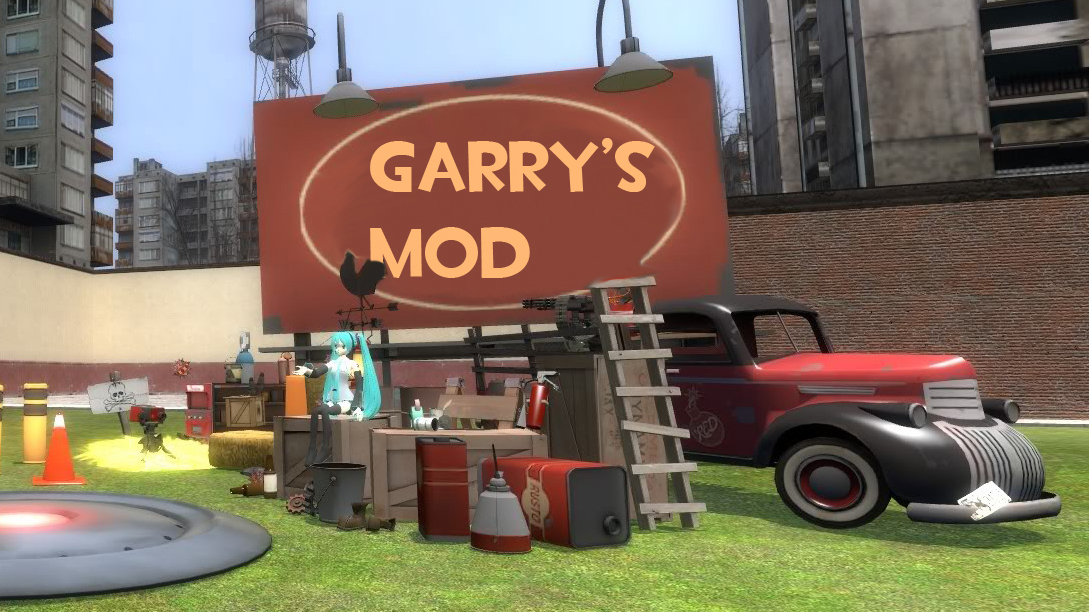
\includegraphics[width=0.8\textwidth]{garrys.jpg}
    \caption{Garry's Mod screenshot.}
    \label{fig:awesome_image}
\end{figure}

It's an open-world game and the differentiating factor from other games is that the game gives the player the possibility to add anything personalized like buildings, weapons and characters, gamemodes and other neat features. All of this is possible using the scripting language called Lua and it allows the user the possibility of coding his own artificial intelligence for any creature as well as any other feature to their own creations.


\subsection{Case Study -  \textit{Minecraft: Pi Edition}}

\textit{Minecraft: Pi Edition} is a version of \textit{Minecraft} developed for the \textit{Raspberry Pi}. It is based on version Alpha 0.6.1 of Pocket Edition but is slightly cut down, containing a revised feature set and support for multiple programming languages. The Pi Edition is intended as an educational tool for novice programmers.

\begin{figure}[h!]
    \centering
    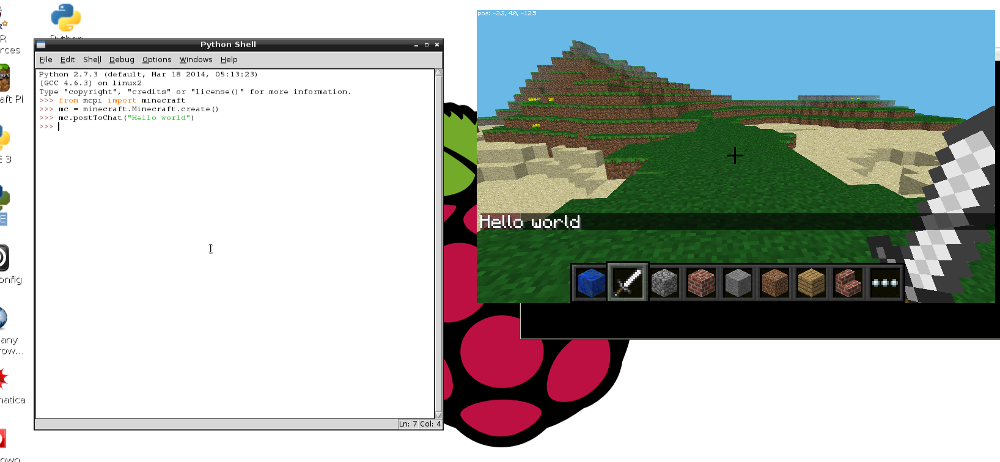
\includegraphics[width=0.8\textwidth]{mine.png}
    \caption{\textit{Minecraft: Pi Edition} screenshot.}
    \label{fig:awesome_image}
\end{figure}

This gives the player the possibility to use a Python programming interface to manipulate the world around you.

\section{Advantages and disadvantages of scripting}
\subsection{Disadvantages}
As useful as they are, conventional scripting languages have syntactic and other limitations, however, which tend to limit their efficiency and expressive power. For instance, they have very limited support for:
\begin{itemize}

  \item Concurrency;
  \item Data structuring;
  \item Information hiding;
  \item Object-oriented programming;
  \item Regular expressions.

\end{itemize} 
Responding to these deficiencies, language developers have created extended scripting languages such as Perl, Python, and Tcl/Tk, among others which evolved to some of the more recent languages we have today.

These languages are still able to invoke and glue together other programs, manipulate files, and set values on-the-fly, but they are also appropriate for writing much larger applications.


\subsection{Advantages}

Up until now we named most of the scripting languages’ strong points in terms of comparison between compiled languages but here are the most “attractive” ones: 
\begin{itemize}
  \item Flexibility of typelessness;
  \item Rapid turnaround of interpretation;
  \item Higher level semantics;
  \item Appropriateness for gluing components and internet programming;
  \item Ease of learning and increase in amount of casual programming.
\end{itemize} 


\emph{\\“Scripting and system programming are symbiotic. Used together, they produce programming environments of exceptional power.” }

\emph{by: }John K. Ousterhout Sun Microsystems Laboratories

Scripting: HigherLevel Programming for the 21st Century\\

In game development we see this in a great variety of cases naming even some of the big names in gaming industry, such as \textit{Riot Games}, \textit{Valve}, \textit{Crytek} and \textit{Blizzard Entertainment}.

With the use of scripting languages (in many cases Lua and Squirrel) companies were able to “glue” some of the core components in their games providing them with new and amazing ways to play their games. One of the best examples available is Garry’s Mod, a game that is purely made out of mod’s, in other words, this game in made from separate game worlds built on top of the core game engine which gives the developers access to all the engine’s functionality through script programming. 

The game even provides its own mod called “Sandbox” where users call experiment with all the resources available in the game and make their own world and through scripting. This becomes very simple and efficient because every change can be made instantly in runtime.

\section{Conclusion}
Having researched a fair amount on many and not so much diverse scripted languages we encountered some of the main aspects that make these languages have such a strong presence in the gaming industry, why they’re making a comeback since their creation and what distinguishes them from the more popular compiled languages.

When starting the creation of a new game and you want to follow the choices of the giants of gaming market you should go for Lua scripting language, with a engine written in C/C++.

With this we were inspired to create some content of our own using scripted languages.

\section{References}
\begin{description}
\item Eyal Oren and Renaud Delbru, \emph{ActiveRDF: object-oriented RDF in Ruby}, \url{http://ceur-ws.org/Vol-181/paper2.pdf}.
\item Scripting Languages, \emph{Rich Morin and Vicki Brown}, \url{http://www.mactech.com/articles/mactech/Vol.15/15.09/ScriptingLanguages/index.html}.
\item John K. Ousterhout Sun Microsystems Laboratories, \emph{Scripting: HigherLevel Programming for the 21st Century}, \url{http://web.stanford.edu/~ouster/cgi-bin/papers/scripting.pdf}.
\item Ronald P. Loui, \emph{In Praise of Scripting:  Real Programming Pragmatism}, \url{http://www.cse.wustl.edu/~loui/praiseieee.html}.
\item Lua, \emph{Lua Scripting Language}, \url {http://www.lua.org/}.
\item Raspberry Pi, \emph{Minecraf: Pi Edition}, \url{http://www.raspberrypi.org/resources/learn/}
\item Garry's Mod, \emph{Garry’s Mod Lua Tutorials}, \url{http://wiki.garrysmod.com/page/Category:Lua_Tutorials}


\end{description}
\end{document}
